\section{Booking}
I dette afsnit beskrives design og implementering af Booking widgetten med fokus på de US's der omhandler at oprette/slette/redigere ressourcer(BookingItems) og foretage gentagende reservationer. For et hurtigt overblik over hvordan Booking systemet er blevet udviklet, se figur \ref{fig:Booking_Iterationer}. En uddybende beskrivelse af de forskellige iterationer, og hvorfor der er blevet arbejdet på denne måde, beskrives efterfølgende. 

\begin{figure}[H]
  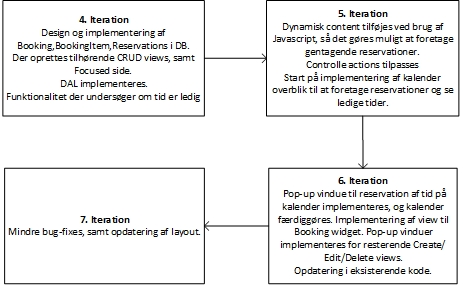
\includegraphics[width=0.8\linewidth]{01_Billeder/10_Design_og_implementering/Booking/Iterationer.jpg}
  \centering
  \caption{Overblik over arbejde i de forskellige iterationer for udvikling af Booking system}
  \label{fig:Booking_Iterationer}
\end{figure} 

\subsection{Opret/slet/redigér ressource(BookingItem)}
\subsubsection{Iteration 4}
Til at starte med tages der udgangspunkt i arkitekturen for databasen. Indledningsvist implementeres Booking og BookingItem. Disse to vælges da de er de mest simple, og skal virke før en reservation af et BookingItem kan foretages. Der implementeres views for at kunne oprette/slette/redigere i Booking, samt BookingItems, i overenstemmelse med figur \ref{fig:Booking_STMResource_Initial}. Når disse er oprettet og tilhørende controller actions implementeret, er US'en der omhandler at kunne oprette/slette/redigere i ressourcer da opfyldt.

\subsection{Iteration 6}
I denne iteration implementeres sådan at de tidligere views der blev oprettet i 4. iteration undtagen Focused, nu vises i et Pop-up vindue. Viewet hvori der tilføjes en ressource, skal kunne tilgås både fra en Booking-widget, samt Focused viewet. Ifølge arkitekturen skal der omdirigeres til viewet som pop-up vinduet blev vist i. Ud fra disse kriterier laves et flowchart der beskriver flowet i POST funktionen for add \ref{fig:Flowchart_AddResource}.   

\begin{figure}[H]
  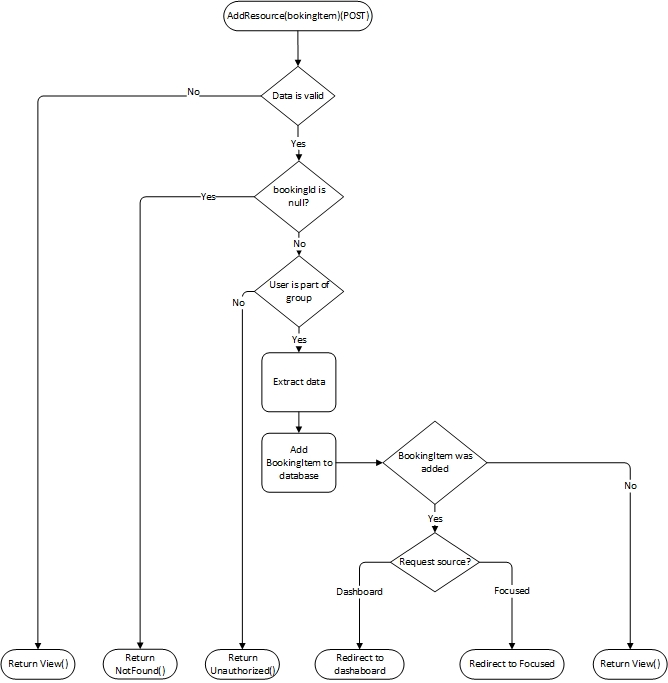
\includegraphics[width=0.9\linewidth]{01_Billeder/10_Design_og_implementering/Booking/Flow_AddResource.jpg}
  \centering
  \caption{Flowchart der viser flowet i koden for AddResource(POST) funktionen i BookingController}
  \label{fig:Flowchart_AddResource}
\end{figure}


\subsection{Foretag gentagende reservationer}
\subsubsection{Iteration 5}
Når det er muligt at foretage enkelte reservationer, og det sikres at disse ikke kan overlappe, implementeres Javascript der gør det muligt at foretage gentagende reservationer, i overensstemmelse med figur \ref{fig:Booking_STMReservation_Initial}. Når der foretages en enkelt reservation eller en gentagende reservation, kaldes den samme Action i controlleren da der anvendes en 'form' til at sende data tilbage med. Funktionen i controlleren skal derfor designes så den kan håndtere dette. Der laves et flowchart for denne Action som skal beskrive hvordan flowet i koden forløber alt efter hvilke informationer den får. Dette kan ses på figur \ref{fig:Booking_FlowCreateReservation}. 

\begin{figure}[H]
  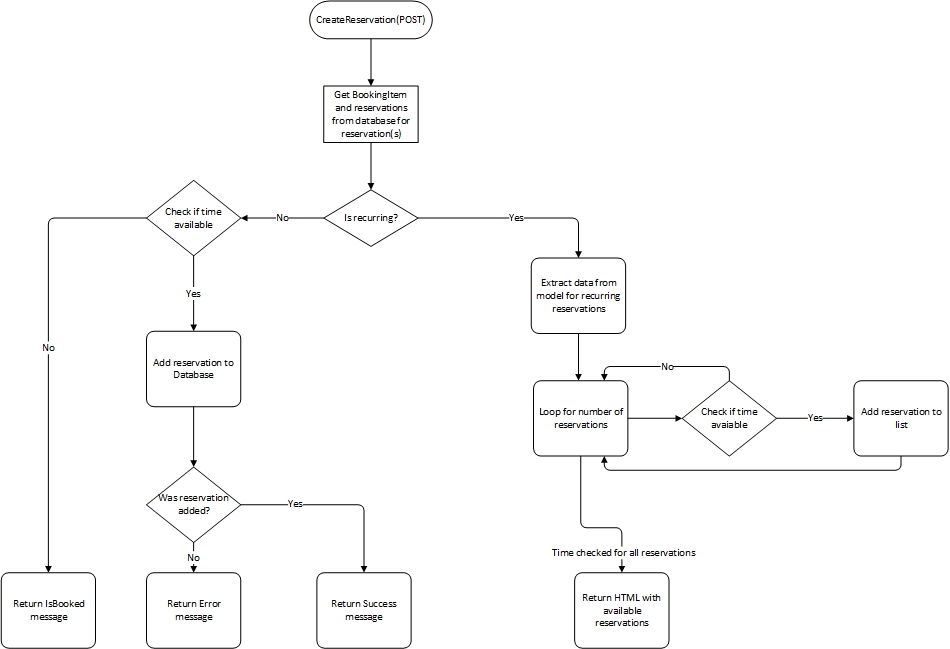
\includegraphics[width=\linewidth]{01_Billeder/10_Design_og_implementering/Booking/Flowchart_ServerCreateReservation.jpg}
  \centering
  \caption{Flowchart der beskriver flowet i koden i CreateReservation(Reservation)(POST). Nederste niveau indikerer slutningen på flowet.}
  \label{fig:Booking_FlowCreateReservation}
\end{figure}

\jonathan{Jeg synes du skal gøre billedet mindre i Visio og så gøre det lidt større her i rapporten. Den højre del kan måske trækkes lidt tættere sammen med det andet?}

Ud fra svaret fra controlleren, reagerer Javascriptet i browseren. Hvis en besked modtages som fx "IsBooked" opdateres siden med en fejlbesked. Hvis der returneres en URL fx /Booking/Focused/1223 omdirigeres til denne side. Hvis HTML returneres, tilføjes denne til den nuværende side. Et flowchart der beskriver flowet i koden hos klienten kan ses på figur \ref{fig:Booking_FlowClientCreateReservation}.  

\begin{figure}[H]
  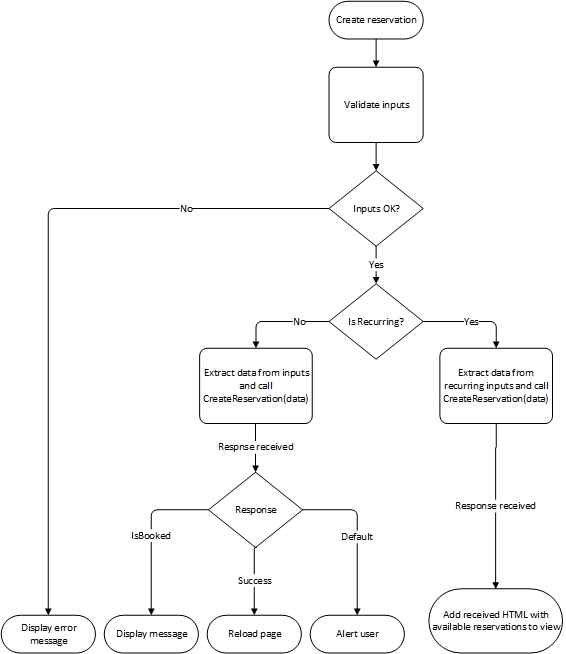
\includegraphics[width=\linewidth]{01_Billeder/10_Design_og_implementering/Booking/FlowChart_ClientCreateReservation.jpg}
  \centering
  \caption{Flowchart der beskriver flowet i Javascript koden der kører i browseren når brugeren trykker på Create reservation knappen}
  \label{fig:Booking_FlowClientCreateReservation}
\end{figure}

Når brugeren har fået overblik over de mulige gentagende reservationer, og er tilfreds kan han/hun da bekræfte de mulige reservationer. Dette kalder nu ConfirmRecurringReservations() POST funktionen i Booking-Controlleren. Her laves der også et flowchart der viser forløbet i koden. Denne kan ses på figur \ref{fig:Booking_FlowConfirmRecurring}.   

\begin{figure}[H]
  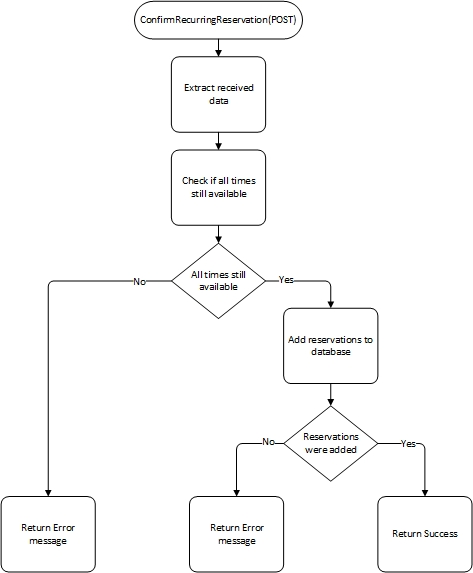
\includegraphics[width=0.8\linewidth]{01_Billeder/10_Design_og_implementering/Booking/Flowchart_ServerConfirmReservation.jpg}
  \centering
  \caption{Flowchart der beskriver flowet i koden i ConfirmRecurringReservation()(POST). Her ses det at der undersøges om andre brugere har reserveret den pågældende ressource i mellemtiden. Hvis der er dette, returneres en fejlmeddelelse, som vises til brugeren.}
  \label{fig:Booking_FlowConfirmRecurring}
\end{figure}
 Med denne implementering er det muligt at foretage en gentagende reservation af en ressource. 

\subsubsection{Iteration 6}
I denne iteration tilføjes alle de nødvenige Pop-up vinduer som beskrevet i arkitekturen for Booking. Desuden implementeres viewet til widgetten på dashboard siden. Designet for dette er ikke vist her, da det der tilføjes er magen til det som blev tilføjet til funktionen, hvor der oprettes en ressource.

\subsection{Øvrige US's}
Til implementering af de øvrige US's anvendes meget af den samme tankegang og fremgangsmåder som i de to ovenstående US's. Indledningsvist implementeres grundfunktionaliteten, hvorefter der tilføjes pop-up vinduer, og designet gøres pænere. Under implementeringen af kalenderen, hentes der dog ikke noget HTML til et pop-up vindue fra serveren. Denne sendes med ud første gang, og Javascriptet sørger for at opdatere denne pop-up alt efter hvilken tid som brugeren klikker på. På denne måde spares flere kald til serveren og hastigheden øges. 



















